% !TeX encoding=utf8
% !TeX spellcheck = de_DE
% !TeX root = ../Diploma.tex

\chapter{Konzept des Servers}\label{sec:conceptServer}
Inhalt dieses Kapitels soll die Planung sein, welche für die Umsetzung des RESTful Schachservers benötigt wird. Dabei dient der erste Abschnitt zur Erläuterung der Anforderungen, welche der Server mitbringen bzw. erfüllen soll. Enthalten ist dabei auch eine Erläuterung der benötigten Ressourcen. Der zweite Abschnitt dieses Kapitels befasst sich anschließend damit, wie der Zugriff auf einzelne Ressourcen des \gls{REST}-Servers erfolgen soll. Dabei werden alle möglichen Request-Methoden für die jeweiligen Ressourcen näher beleuchtet. Abschließend wird erläutert, wie das Designkonzept HATEOAS in dieser Anwendung erreicht werden soll.

\section{Anforderungen}\label{sec:anforderungen}
Die Grundanforderungen an den RESTful Schachserver sollen in erster Linie die Bereitstellung aller benötigten Ressourcen sein. Dabei sollen Elemente erstellt, ggf. bearbeitet und gelöscht werden können. Zusätzlich soll die Möglichkeit bestehen, einzelne oder alle gespeicherten Elemente einer Ressource abzufragen. Beim Erstellen eines neuen Ressourcenelements soll dieses in einer SQLite Datenbank gespeichert und die ID automatisch durch SQLite generiert werden.\\
\\
Um ein Schachspiel abzubilden, bedarf es dabei der Ressourcen Player (Spieler), Match (Partie) und Draw (Zug), welche in den nachfolgenden \hyperref[sec:resplayer, sec:resdraw]{Unterabschnitten~\ref{sec:resplayer} bis \ref{sec:resdraw}} näher betrachtet werden.\\
\\
Als abschließende Anforderung ist noch die Fehlerresistenz zu erwähnen. Denn die im Rahmen dieser Arbeit entstandene Praktikumsaufgabe\footnote{siehe \hyperref[chap:Appendix:A]{Anhang~\ref{chap:Appendix:A}}} soll durch zukünftige Studenten bearbeitet werden, wobei der Server als Grundlage dienen soll.\\
\\
Zur Unterstützung der Erläuterungen in den \hyperref[sec:resplayer, sec:resdraw]{Kapiteln~\ref{sec:resplayer} bis \ref{sec:resdraw}} bietet die \hyperref[fig:classdiagram]{Abbildung~\ref{fig:classdiagram}}, in Form eines \gls{UML} Klassendiagramms, eine Veranschaulichung.
\begin{sidewaysfigure}
	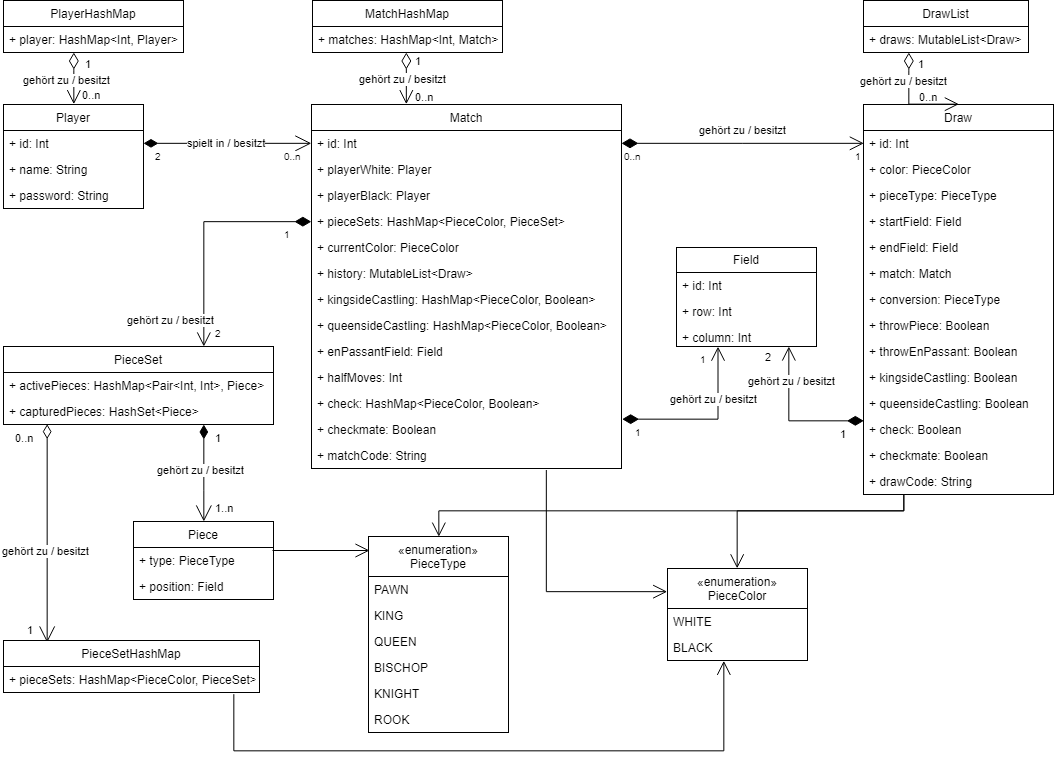
\includegraphics[width=0.9\textwidth]{images/classdiagram.png}
	\caption{Klassendiagramm: Modelle des Servers}
	\label{fig:classdiagram}
\end{sidewaysfigure}

\subsection{Ressource: Player (Spieler)}\label{sec:resplayer}
Neben der ID, welche schon im Abschnitt \ref{sec:anforderungen} erwähnt und durch die SQLite Datenbank generiert werden soll, besitzt der Player noch Informationen über seinen Namen und sein Passwort.\\
\\
Nach dem Anlegen eines neuen Players soll eine Änderung des Passwortes möglich, aber die des Namens nicht möglich sein.

\subsection{Ressource: Match (Partie)}\label{sec:resmatch}
Neben der ID besitzt ein Match Informationen über die beiden Spielteilnehmer und deren Figurenstellung auf dem Schachbrett. Zusätzlich wird registriert, welcher der beiden Player als nächstes seinen Zug tätigen muss, welche Möglichkeiten zum rochieren bestehen, ob ein Schlag \enquote{en passant} möglich ist und wenn ja auf welches Feld gezogen werden muss und wie viele Halbzüge gespielt wurden. Der Wert der Halbzüge wird dabei zurückgesetzt, sobald eine Bauernfigur gezogen oder eine beliebige Figur geschmissen wurde. Zusätzlich kann über ein Match ermittelt werden, ob ein Spieler im Schach steht oder ob das Spiel schon bis zum Schachmatt gespielt wurde. All diese Informationen werden zusätzlich noch als String in der \gls{FEN}\footnote{\label{foot:chapter}siehe \hyperref[sec:chessNotation]{Kapitel~\ref{sec:chessNotation}}} gespeichert.

\subsection{Ressource: Draw (Zug)}\label{sec:resdraw}
Die Ressource Draw speichert zusätzlich zur ID die Farbe des Spielers, die Art der Spielfigur, Start- und Endfeld des Zuges, ob eine Figur geschlagen wurde, wenn ja ob durch \enquote{en passant} und ob seitens der Dame oder des König rochiert wurde. Diese Informationen werden ähnlich zum Match als String aber in diesem Fall in der \gls{SAN}\footref{foot:chapter} gespeichert.

\section{Ressourcenzugriffe mithilfe von Controllern}
Die einzelnen Zugriffe auf die Ressourcen werden in den \hyperref[sec:rootController, sec:errorController]{Kapiteln~\ref{sec:rootController} bis \ref{sec:errorController}} nach ihrer Art bzw. deren Aufgaben in einzelne Controller unterteilt, um eine gute Übersicht zu wahren. Für alle Einstiegspunkte der \gls{REST}-\gls{API} soll die Request-Methode \code{OPTIONS} bereitstehen, über den ermittelt werden kann, welche Methoden für den jeweiligen Einstiegspunkt zur Verfügung stehen.\\
\\
Etwaige Requestparameter sollen in den Formaten \gls{JSON} oder x-www-form-urlencode an den Request übergeben werden können. Gesendeten Anfragen sollen anschließend ihr Feedback je nach Wunsch des Clients, via Content Negotiation, entweder in der \gls{JSON} oder als \gls{XML} zurückgeben. Dafür sind drei Strategien zur Umsetzung bereitzustellen, entweder mittels Suffix, einem URL-Parameter oder dem \gls{HTTP} Accept-Header. 

\subsection{Root Controller}\label{sec:rootController}
Mit dem Root Controller soll der Einstiegspunkt an der \gls{URI} \code{/api} bereitgestellt werden. Ein GET-Request an diesem Einstiegspunkt soll aber ausschließlich Links zu den einzelnen Startpunkten der Ressourcen Player, Match und Draw bereitstellen. Dies wiederum dient der Umsetzung des Konzeptes HATEOAS, welches im \hyperref[sec:konzeptHATEOAS]{Kapitel~\ref{sec:konzeptHATEOAS}} genauer definiert wird und ausführlichere Erläuterungen enthält, wie das Ziel dieses Konzeptes erreicht werden soll.\\
\\
Die nachfolgende \hyperref[fig:rootController]{Abbildung~\ref{fig:rootController}} dient dabei als Veranschaulichung des Einstiegspunktes.\\
\begin{figure}[htb]
	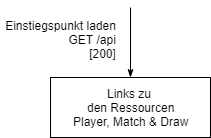
\includegraphics[width=0.323\textwidth]{images/root-controller.png}
	\caption{Root Controller - Übersicht der Einstiegspunkte}
	\label{fig:rootController}
\end{figure}

\subsection{Player Controller}\label{sec:playerController}
Der Player Controller soll zwei Einstiegspunkte an den \glspl{URI} \code{/api/players} und \code{/api/players/\{id\}} zur Verfügung stellen. Der Parameter \code{\{id\}} dient dabei als Platzhalter für die ID eines Players.\\
\\
Am ersten Einstiegspunkt ist eine Liste aller Spieler über einen GET-Request bereitzustellen. Des Weiteren soll an diesem die Möglichkeit bestehen, einen neuen Player mithilfe eines POST-Requests zu erzeugen. Dabei muss als Parameter der Name und das Passwort des Players mitgegeben werden. Die ID ist durch die SQlite-Datenbank mittels Autoincrement zu erzeugen. Bei erfolgreicher Erstellung des Players ist dieser als \gls{HTTP}-Response zurück zugegeben. Tritt bei diesem Prozess jedoch ein Fehler auf so muss, anstatt des Players, dieser zurück gegeben werden.\\
\\
Am zweiten Einstiegspunkt ist ein einzelner existierender Player über einen GET-Request bereitzustellen, über einen DELETE-Request gelöscht und über einen PATCH-Request aktualisiert werden können. Dabei darf bei einer Aktualisierung eines Players nur das Passwort, laut Anforderungen\footnote{siehe \hyperref[sec:anforderungen]{Kapitel~\ref{sec:anforderungen}}}, geändert werden.\\
\\
Für ein besseres Verständnis der einzelnen Einstiegspunkte, mit den dazugehörigen Request-Methoden, bietet die \hyperref[fig:playerController]{Abbildung~\ref{fig:playerController}} eine visuelle Verdeutlichung des Player Controllers.\\
\begin{figure}[htb]
	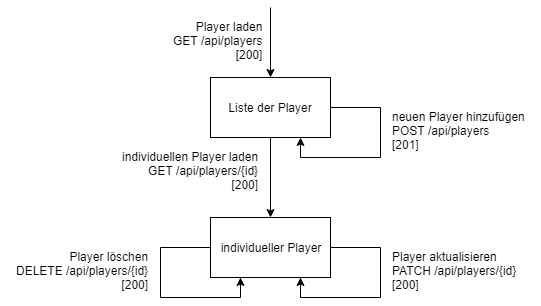
\includegraphics[width=0.816\textwidth]{images/player-controller.png}
	\caption{Player Controller - Übersicht der Einstiegspunkte}
	\label{fig:playerController}
\end{figure}

\subsection{Match Controller}\label{sec:matchController}
Die \glspl{URI} \code{/api/matches}, \code{/api/matches/\{id\}}, \code{/api/matches/\{id\}/draws} und \code{/api/matches/\{id\}/pieceSets} sollen durch den Match Controller bereitgestellt werden.\\
\\
Dabei dient die erste \gls{URI} ebenso wie beim Player Controller der Zurverfügungstellung einer Liste aller registrierten Matches und dem Anlegen neuer. Das Bereitstellen der Liste hat mittels GET- und das Anlegen mittels POST-Request zu erfolgen. Der GET-Request soll zwei optionale boolesche Parameter bereitstellen, womit das Senden der Historie von Draws bzw. der Figurenstellung bestimmt wird. Standardmäßig sollen die beiden Parameter \code{true} sein. Nachfolgend wird genauer erläutert wie diese Informationen separat angefordert werden können. Um ein neues Match zu registrieren, müssen dabei die ID's der beiden Spielteilnehmer als Parameter mitgesendet werden. Anhand des Parameternamens wird festgelegt, welcher Spieler Weiß und welcher Schwarz spielt.\\
\\
Der zweite Einstiegspunkt in diesem Controller soll ausschließlich dazu verwendet werden, um einzelne Matches mithilfe eines GET-Request anzufordern oder mit einem DELETE-Request zu löschen. Für das Anfordern eines einzelnen Matches stehen dabei, ebenso wie beim Request einer Match-Liste, zwei boolesche Parameter bereit. Sollte ein Nutzer ein Match löschen, so sind die zugehörigen Draws automatisch mit zu löschen. Um eine unrechtmäßige Manipulation der Match-Daten durch einen Nutzer zu verhindern, soll keine Möglichkeit bereitstehen, ein Match direkt zu aktualisieren. Änderungen der Match-Daten dürfen ausschließlich über das Hinzufügen von neuen Draws\footnote{siehe \hyperref[sec:drawController]{Kapitel~\ref{sec:drawController}}} erfolgen.\\
\\
Die letzten beiden Einstiegspunkte sollen dazu dienen, große Match bezogene Daten separat zu ermitteln. Dabei ist mittels GET-Request an der \gls{URI} \code{/api/matches/\{id\}/draws} eine Liste aller Draws und über die \gls{URI} \code{/api/matches/\{id\}/pieceSets} eine Map mit allen Figuren der beiden Spielteilnehmer bereitzustellen. Neben den aktuell auf dem Spielfeld stehenden Figuren sollen dabei auch die Daten der bereits Geschmissenen mitgeschickt werden.\\
\\
Die \hyperref[fig:matchController]{Abbildung~\ref{fig:matchController}} bietet für die zuvor definierten Einstiegspunkte eine grafische Veranschaulichung.\\
\begin{figure}[htb]
	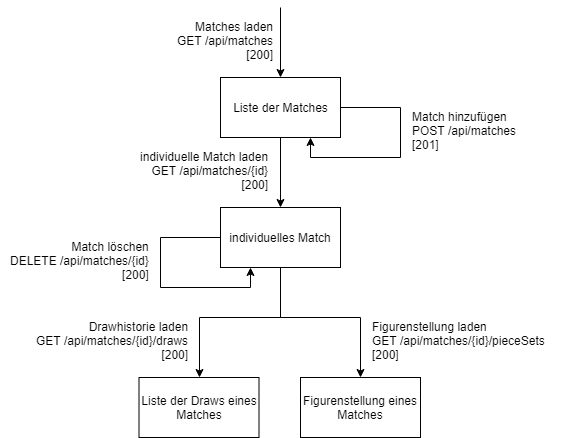
\includegraphics[width=0.85\textwidth]{images/match-controller.png}
	\caption{Match Controller - Übersicht der Einstiegspunkte}
	\label{fig:matchController}
\end{figure}

\subsection{Draw Controller}\label{sec:drawController}
Auch der Draw Controller stellt wieder zwei Einstiegspunkte an den \glspl{URI} \code{/api/draws} und \code{/api/draws/\{id\}} bereit. \\
\\
Am ersten Einstiegspunkt soll dabei wieder eine Liste mittels GET- und das Hinzufügen mittels POST-Request von Draws zur Verfügung gestellt werden. Für das Hinzufügen eines neuen Draws ist die ID des Matches und der Draw-Code in der \gls{SAN} als Parameter notwendig. Zusätzlich soll die Möglichkeit bestehen, die Zeilen- und Spaltennummer der Startposition mitzugeben. Wenn diese Informationen nicht mitgegeben werden, soll der Controller die Startposition kalkulieren. Spalten sind dabei als Nummern und nicht als Buchstaben zu übergeben\footnote{A $\rightarrow$ 1; B $\rightarrow$ 2; C $\rightarrow$ 3; D $\rightarrow$ 4; E $\rightarrow$ 5; F $\rightarrow$ 6; G $\rightarrow$ 7; H $\rightarrow$ 8}. Nach erfolgreicher Validierung des Draw-Codes soll der Draw dem zugehörigen Match hinzugefügt und die Match-Daten aktualisiert werden.\\
\\
Über den zweiten Einstiegspunkt soll die Abfrage nach einem einzelnen Draw möglich sein, aber eine Löschung oder Aktualisierung nicht. Sonst wäre eine Manipulation der Match-Daten seitens des Nutzers möglich. Die Entfernung von Draws ist ausschließlich über die Löschung des dazugehörigen Matches\footnote{siehe \hyperref[sec:matchController]{Kapitel~\ref{sec:matchController}}} zu erfolgen.\\
\\
Wie in den vorherigen Kapiteln bietet die \hyperref[fig:drawController]{Abbildung~\ref{fig:drawController}} ein Veranschaulichung der definierten Einstiegspunkte.\\
\begin{figure}[htb]
	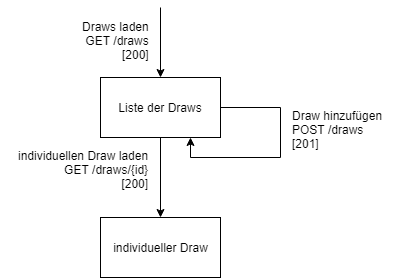
\includegraphics[width=0.7735\textwidth]{images/draw-controller.png}
	\caption{Draw Controller - Übersicht der Einstiegspunkte}
	\label{fig:drawController}
\end{figure}

\subsection{Error Controller}\label{sec:errorController}
Mithilfe des Error Controllers muss gewährleistet werden, dass alle nicht in der \gls{REST}-\gls{API} definierten Einstiegspunkte bzw. nicht definierte Request-Methoden an den Einstiegspunkten abgefangen werden. Tritt ein solcher Fall auf, so ist ein Fehler vom Server zurück zugeben. Somit wird verhindert, dass ein Nutzer der \gls{API} einen Serverfehler, mit dem HTTP-Statuscode \code{500}\footnote{siehe \cite[A.2.5]{kretzschmar}}, zurückerhält.

\section{Erreichung des Designkonzepts HATEOAS}\label{sec:konzeptHATEOAS}
Um das Ziel der Selbstbeschreibung, welches das Konzept HATEOAS verfolgt, zu erreichen, gibt es mehrere Lösungswege.\\
\\
Zum einen besteht die Möglichkeit der Erweiterung einer Ressource, wodurch diese als Hypermedia Format angesehen werden kann. Ein Beispiel dafür ist die \gls{HAL}, welche in der Spezifikation \cite{halSpezification} definiert wurde. Diese stellt mittels eines Dialektes der \gls{JSON} die \gls{MIME} Typen \code{application/hal+json} und \code{application/hal+xml} bereit, wodurch Ressourcen mit Relationen, in Form von Hyperlinks, ergänzt werden können.\\
\\
Eine weitere Lösungsvariante kann durch den Link-Header des \gls{HTTP}-Response realisiert werden. Diesem kann einfach eine Menge von Links in Form eines Strings übergeben werden, welchen der Client anschließend auswerten kann.\\
\\
Welche Variante die bessere ist, liegt im Auge des Betrachters. Für die Implementierung des Schach-Servers wurde Variante zwei gewählt, weil dadurch die Trennung der Links und der eigentlichen Ressource strikter wahrgenommen werden kann. Auch Kai Spichale bevorzugt diese Variante, denn dieser betrachtet die Links in seinem Buch \cite[158]{apiDesign} als Metainformationen und diese gehören seiner Meinung nach nicht in die Ressource.